\documentclass[iop, twocolappendix, numberedappendix, tighten, appendixfloats]{emulateapj}
\citestyle{apj}

\usepackage[stable]{footmisc}
\usepackage{graphicx}
\usepackage{hyperref}
\usepackage{txfonts}
%\usepackage{hyperref}
\usepackage{natbib}
\bibpunct[, ]{(}{)}{;}{a}{}{,}
%\bibliographystyle{./bibtex/apj}

\newcommand{\farc}{\hbox{$.\!\!^{\prime\prime}$}} 
\newcommand{\ergA}{$\rm{erg\,cm^{-2}\,s^{-1}\,\AA^{-1}}$} 
\newcommand{\erg}{$\rm{erg\,cm^{-2}\,s^{-1}}$} 
\newcommand{\kms}{$\rm{km\,s^{-1}}\,$}

\newcommand{\griz}{$g' r' i' z'$}
\newcommand{\JHK}{$JHK_{\rm{s}}$}
\newcommand{\gK}{$g' r' i' z' JHK_{\rm{s}}$}
\newcommand{\Msun}{$M_\odot$}
\newcommand{\lya}{Ly$\alpha$} 
\newcommand{\lyb}{Ly$\beta$} 
\newcommand{\lyg}{Ly$\gamma$} 
\newcommand{\hb}{H$\beta$} 
\newcommand{\ha}{H$\alpha$} 
\newcommand{\hg}{H$\gamma$} 
\newcommand{\hi}{\ion{H}{1}} 
\newcommand{\hei}{[\ion{He}{1}]} 
\newcommand{\oi}{[\ion{O}{1}]} 
\newcommand{\sii}{[\ion{S}{2}]} 
\newcommand{\siii}{[\ion{S}{3}]} 
\newcommand{\oii}{[\ion{O}{2}]} 
\newcommand{\oiii}{[\ion{O}{3}]}
\newcommand{\nii}{[\ion{N}{2}]} 
\newcommand{\nv}{[\ion{N}{5}]} 
\newcommand{\neiii}{[\ion{Ne}{3}]} 
\newcommand{\NIii}{[\ion{Ni}{2}]} 
\newcommand{\feii}{\ion{Fe}{2}} 
\newcommand{\civ}{\ion{C}{4}} 
\newcommand{\cii}{\ion{C}{2}}
\newcommand{\mgi}{\ion{Mg}{1}} 
\newcommand{\mgii}{\ion{Mg}{2}} 
\newcommand{\ali}{\ion{Al}{1}} 
\newcommand{\alii}{\ion{Al}{2}} 
\newcommand{\aliii}{\ion{Al}{3}} 
\newcommand{\SIii}{\ion{Si}{2}} 
\newcommand{\SIiv}{\ion{Si}{4}} 
\newcommand{\znii}{\ion{Zn}{2}} 
\newcommand{\crii}{\ion{Cr}{2}} 
\newcommand{\mnii}{\ion{Mn}{2}} 
\newcommand{\tiii}{\ion{Ti}{2}} 
\newcommand{\caii}{\ion{Ca}{2}} 

\usepackage{todonotes}

\begin{document}
	
	\title{\vspace{-0.5cm}The X-shooter GTO sample of GRB afterglow and host Galaxy spectra}
	\altaffiltext{$^{\dag}$}{Based on observations collected at the European Southern Observatory, Paranal, 
		Chile, Program ID: 084.A-0260, 085.A-009, 086.A-0073, 087.A-0055.}
	
	\author{
		J.~Selsing\altaffilmark{1}, 
		D.~Malesani\altaffilmark{1}, 
		T.~Kr\"{u}hler\altaffilmark{1}, 
		P.~Goldoni\altaffilmark{14}, 
		J.~P.~U. Fynbo\altaffilmark{1}, 
		A.~de~Ugarte~Postigo\altaffilmark{11}, 
		J.~Japelj\altaffilmark{20},
		P.~D'Avanzo,
		Z.~Cano,
		S.~Covino\altaffilmark{10}, 
		V.~D'Elia\altaffilmark{7, 12}, 
		H.~Flores,
		O.~E.~Hartoog\altaffilmark{6},
		J.~Hjorth\altaffilmark{1}, 
		P.~Jakobsson\altaffilmark{5}, 
		A.~Levan,
		A.~Melandri,
		S.~Piranomonte \altaffilmark{7},
		R.~S\'anchez-Ram\'irez\altaffilmark{11},
		S.~Schulze\altaffilmark{17, 18}, 
		N.~R.~Tanvir\altaffilmark{19},
		C.~Th{\"o}ne,
		S.~D.~Vergani\altaffilmark{7, 8},
		P.~M.~Vreeswijk\altaffilmark{3}, 
		D.~J.~Watson\altaffilmark{1},
		K.~Wiersema\altaffilmark{19},
		D.~Xu\altaffilmark{1}
		L.~Christensen\altaffilmark{1},
		A.~De~Cia\altaffilmark{3}, 
		L.~Kaper\altaffilmark{6}, 
		L.~A.~Antonelli,
		F.~Fiore,
		A.~Gomboc,
		P.~Groot,
		F.~Hammer,
		C.~Ledoux\altaffilmark{2}, 
		E.~Maiorano,
		B.~Milvang-Jensen\altaffilmark{1}, 
		E.~Palazzi,
		E.~Pian,
		J.~Schaye,
		G.~Tagliaferri\altaffilmark{7},
		R.~A.~M.~J.~Wijers\altaffilmark{6}
	}
	
	\altaffiltext{1}{Dark Cosmology Centre, Niels Bohr Institute, University of Copenhagen, Juliane Maries Vej 30, 2100 K\o benhavn \O, Denmark}
	\altaffiltext{2}{European Southern Observatory, Alonso de C\'{o}rdova 3107, Vitacura, Casilla 19001, Santiago 19, Chile}
	\altaffiltext{3}{Department of Particle Physics and Astrophysics, Faculty of Physics, Weizmann Institute of Science, Rehovot 76100, Israel}
	\altaffiltext{4}{Th\"uringer Landessternwarte Tautenburg, Sternwarte 5, 07778 Tautenburg, Germany}
	\altaffiltext{5}{Centre for Astrophysics and Cosmology, Science Institute, University of Iceland, Dunhagi 5, IS-107 Reykjavik, Iceland}
	\altaffiltext{6}{Astronomical Institute Anton Pannekoek, University of Amsterdam, Science Park 904, NL-1098 XH Amsterdam, the Netherlands}
	\altaffiltext{7}{INAF-Osservatorio Astronomico di Roma, Via Frascati 33, I-00040 Monteporzio Catone, Italy}
	\altaffiltext{8}{GEPI-Observatoire de Paris, CNRS UMR 8111, Univ. Paris-Diderot, 5 Place Jules Janssen - 92190 Meudon, France}
	\altaffiltext{9}{American River College, Physics and Astronomy Dpt., 4700 College Oak Drive, Sacramento, CA 95841, USA}
	\altaffiltext{10}{INAF, Osservatorio Astronomico di Brera, Via E. Bianchi 46, I-23807 Merate, Italy}
	\altaffiltext{11}{Instituto de Astrof\'{\i}sica de Andaluc\'{\i}a (IAA-CSIC), Glorieta de la Astronom\'{\i}a s/n, 18008, Granada, Spain}
	\altaffiltext{12}{ASI-Science Data Centre, Via Galileo Galilei, I-00044 Frascati, Italy}
	\altaffiltext{13}{Institute of Experimental and Applied Physics, Czech Technical University in Prague, Horska 3a/22, 128 00 Prague 2, Czech Republic}
	\altaffiltext{14}{APC, Astroparticules et Cosmologie, Universite Paris Diderot, CNRS/
		IN2P3, CEA/Irfu, Observatoire de Paris, Sorbonne Paris Cite, 10, Rue Alice Domon et L
		eonie Duquet, 75205 Paris Cedex 13, France}
	\altaffiltext{15}{Max-Planck-Institut f\"{u}r extraterrestrische Physik, Giessenbachs
		tra\ss e, 85748 Garching, Germany}
	\altaffiltext{16}{Universit\`a degli studi di Milano-Bicocca, Piazza della Scienza 3,
		20126, Milano, Italy}
	\altaffiltext{17}{Pontificia Universidad Cat\'{o}lica de Chile, Departamento de Astro
		nom\'{\i}a y Astrof\'{\i}sica, Casilla 306, Santiago 22, Chile}
	\altaffiltext{18}{Millennium Center for Supernova Science}
	\altaffiltext{19}{Department of Physics and Astronomy, University ofLeicester, University Road, Leicester, LE1 7RH, UK}
	\altaffiltext{20}{University of Ljubljana,Department of Physics,Faculty of Mathematics \& Physics,SI}\
	
	\begin{abstract}
	The {\it Swift} satellite allows us to use gamma-ray bursts (GRBs) to peer into 
	the hearts of star forming galaxies through cosmic time. Our open
	collaboration, representing most of the active ESO member researchers in this
	field, seeks to build a public legacy sample of GRB X-shooter spectroscopy
	while {\it Swift} continues to fly. We propose to continue our programme to target
	all suitably observable GRB afterglows (up to 15 bursts per semester), with the
	primary goal of producing a well-defined, homogeneous, statistically useful
	sample. To date, our spectroscopy covers a redshift range from 0.059 to about
	8, with more than 20 robust metallicity measurements from absorption lines (over 
	the redshift range 1.7--5.9) and 4 secure detections of H$_2$ or CH molecular
	absorption. Such information is extremely difficult to obtain by other means.
	In terms of studying the spread and redshift evolution in gas-phase properties, the
	sample is still limited by low-number statistics. 
	\end{abstract}
	
	\keywords{Gamma-ray burst: individual: GRB~120815A --- galaxies: high-redshift --- ISM: molecules --- dust, extinction }
	
	\section{Introduction}
	
	
	Only after observing more than 12000 damped Lyman-$\alpha$ absorbers (DLAs)
	towards about 10$^5$ QSOs have 5 systems with 
	$\log({N_\mathrm{HI}/\mathrm{cm^{-2}}}) > 22$
	been identified (Noterdaeme et al.\ 2012, A\&A, 547, L1). Long GRB afterglow
	spectra, by contrast, reveal such systems in the majority of cases (e.g., Jakobsson et
	al.\ 2006, A\&A, 460, L13; Fynbo et al.\ 2009, ApJS, 185, 526).
	Whereas DLAs towards QSOs are mostly limited to $1.8\lesssim z \lesssim 5$ due
	to the atmospheric  UV-cutoff and increasing Lyman-blanketing at increasing
	redshifts (e.g., Rafelski et al.\ 2014, ApJL, 782, L29), GRBs allow us to see 
	into the hearts of star-forming galaxies over
	the full history of cosmic star formation from $z \approx 0$ to $z > 8$ (e.g.,
	Tanvir et al.\ 2009, Nature, 461, 1254; Salvaterra et al.\ 2009, Nature, 461,
	1258; Jakobsson et al.\ 2012, ApJ, 752, 62). With afterglow spectroscopy
	(throughout the electromagnetic spectrum from X-rays to the sub-mm) we can hence
	characterize the properties of star-forming galaxies over cosmic history in
	terms of  redshifts, metallicities, molecular contents, ISM temperatures,
	UV-flux densities, etc.. This is, however, only possible as long as there are
	satellites in orbit that rapidly and accurately locate GRBs. The currently
	operating \textit{Swift} satellite, launched in 2004 and still fully-functioning,
	allows for very efficient follow-up observations of GRBs due to its
	unprecedented rate, speed and precision of localisations.
	
	%With GTO time on X-shooter we
	%have started building a sample of afterglows with X-shooter spectroscopy.
	%X-shooter is ideal for this with its high efficiency, wide wavelength coverage
	%and spectral resolution sufficient for inferring the fundamental physical
	%parameters just listed.
	
	\smallskip
	\smallskip
	
	{\bf The case for a large sample of GRBs with X-shooter spectroscopy.}
	
	There are
	several unanswered but fundamental questions that must be addressed in order
	to exploit the full potential of GRBs as cosmological probes.
	%Among them: what is the true redshift distribution and corresponding luminosity
	%function of long-duration GRBs?
	More than 50\% of the \textit{Swift} bursts with measured redshift are at $z >
	2$, and  5--10\% are expected to be above $z=5$ (Salvaterra et al. 2008, MNRAS, 380, L45; Salvaterra et al.\ 2012, ApJ, 749,
	68; Jakobsson et al.\ 2012, ApJ, 752, 62; Perley et al.\ 2016, ApJ, 817, 7). 
	A high redshift completeness is
	crucial for our understanding of the link between the number density of GRBs
	per unit redshift and the global star-formation history of the Universe, as
	measured by other means (UV, FIR, sub-mm, see Robertson \& Ellis 2011, ApJ, 744,
	95). The detection of GRBs at $z > 6$ shows that GRBs have become competitive as
	a tool to identifying galaxies at the highest redshifts and unsurpassed in
	providing detailed abundance information via absorption line spectroscopy
	(Tanvir et al.\ 2012, ApJ, 754, 46, McGuire et al.\ 2016, ApJ submitted, 
	arxiv:1512.07808).
	
	\smallskip
	
	%The sample of short GRBs with redshifts remains too small and too
	%incomplete to really
	%constrain their redshift distribution (Guetta \& Piran 2006, A\&A, 453, 823;
	%Salvaterra et al.\ 2008, MNRAS, 388, 6) making it of extreme importance to
	%enlarge as far as possible the number of known redshifts for this class of
	%sources.
	
	From March 2005 to March 2016 there have been about 350 {\it Swift} bursts 
	complying with
	our sample selection criteria (see ``Immediate objective''), and about half of them have
	measured redshifts. Among the latter subset, the team proposing these observations has
	measured about two thirds of the redshifts, mainly with FORS1/2 and X-shooter (see
	Fynbo et al.\ 2009, ApJS, 185, 526;  Jakobsson et al.\ 2012, ApJ, 752, 62;
	Kr\"uhler et al.\ 2012, ApJ, 758, 46). Our current aim is to build a sample superior to
	our previous low-resolution survey (Fynbo et al.\ 2009, ApJS, 185, 526), both in
	terms of quantity and  quality of the spectra. Our program started as 
	guaranteed time observations during
	periods 84-91, and we have continued in open time since then. 
	
	%In P84 we started the X-shooter legacy survey in GTO time. Our aim is to  build
	%a sample of GRBs superior to our previous  low-resolution  survey, Fynbo et al.\
	%2009, ApJS, 185, 526) both in terms of quantity and  quality of the spectra. The
	%last period of GTO time on the survey was P90 (plus 6 hr of leftover GTO time
	%in  P91) and for P92 a proposal like this was  accepted for continuation of the
	%program in open time (concerning P93 see box 8). 
	
	\smallskip
	
	X-shooter is in many ways
	the ideal GRB follow-up instrument and indeed GRB follow-up was one of the
	primary science cases behind the instrument design and implementation. Our
	program secures general purpose GRB afterglow spectroscopic follow-up 
	that adds strong legacy value to the \textit{Swift} GRB sample.
	Due to the wide wavelength range of X-shooter  
	with the same observation cover molecular H$_2$ absorption near the
	atmospheric cut-off and all the strong emission lines from the host in the
	NIR arm (e.g., Friis et al., 2015, MNRAS, 451, 167). In general, the wide wavelength coverage ensures that we always have
	features on which to base a redshift measurement as long as the afterglow is
	brighter than about 23 mag in either the $R$- or $z$-band. 
	Frequently, emission lines are also detected from the underlying host, which
	also provide further information such as SFR and metallicity (the top right 
	panel in Fig.~1 shows an example). Only for 
	7 out of more than 70 secured spectra could we not measure a redshift.   
	With the X-shooter survey we
	provide {\bf metallicity measurements} for about 30\% (Voigt-profile fits)
	of the $z>1.7$ events.
	So far we have
	measured metallicities for more than 20 GRB afterglows with X-shooter.
	With the wide wavelength coverage of X-shooter we can
	study important chemical species as Zn\,\textsc{ii}, Cr\,\textsc{ii} and $\alpha$
	elements over a much wider redshift range than what is possible with other
	instruments.
	As an example, we have measured a metallicity of $0.1 Z_\odot$ for GRB\,100219A
	at $z=4.669$ (Th{\"o}ne et al.\ 2013, MNRAS, 428, 3590), $0.02Z_\odot$ for 
	GRB\,111008A at $z=4.991$ (Sparre et al.\ 2014, ApJ, 785, 150) and $0.05Z_\odot$
	for the $z=5.9125$ GRB\,130606A (Hartoog et al.\ 2015, A\&A, 580, 139).  
	Reconciling the
	abundance patterns of GRB absorbers, other types of absorbers, QSO DLAs
	in particular, and old stars in the Local Group is an important long-term
	goal (see also Sparre et al.\ 2014, ApJ, 785, 150).
	Metallicities are also measured from host emission lines (Kr{\"u}hler et al.\ 2015,
	A\&A, 581, A125).
	GRB spectroscopy also allows us to determine the dust content of their environments,
	both through analysis of the depletion pattern and through measurement of the
	associated extinction (Japelj et al.\ 2015, A\&A, 451, 2050). 
	This allows us to quantify the dust-to-metals ratio and its
	evolution with redshift (e.g., De Cia et al.\ 2013, A\&A, 560, 88; Zafar \&
	Watson 2013, A\&A, 560, 26).
	%Moreover, GRB
	%afterglows allow investigation of random foreground absorbers, complementing
	%QSO sightline studies (e.g., Schulze et
	%al.\ 2012, A\&A, 546, 20).
	
	%In Fynbo et al. (2009, ApJS, 185,
	%526), we compare the host-galaxy HI
	%column density and metallicity (most of which has been measured by our group)
	%with a sample of damped \lya\ systems (DLAs) along QSO sightlines. We show that
	%most GRB-DLAs have a much larger column than QSO-DLAs.  The difference in
	%column density and metallicity for GRB and QSO sightlines shows that the total
	%cross-section for environments like those of GRBs must be less than a few
	%percent of the total cross-section for QSO-DLAs, and suggests that GRB
	%sightlines probe regions with high gas density.
	
	%The issue of production and {\bf release of Lyman continuum radiation} is
	%currently not fully understood, but the evidence suggests that star-forming
	%galaxies are dominating, in particular at the highest redshifts (e.g., Bianchi
	%et al.\ 2001, A\&A, 376, 1; Chen et al.\ 2007, ApJ, 667, L25). Also here
	%X-shooter spectroscopy will allow major progress due to the excellent blue
	%sensitivity.
	
	%GRB afterglows can probe dust in high-redshift star-forming galaxies
	%including exploring the {\bf 2175~\AA{} extinction bump}
	%(El\'iasd\'ottir et al.\ 2009, ApJ, 697, 1725; Zafar et al.\ 2011, A\&A,
	%732, 143).
	%Due to the broad wavelength  coverage we can do
	%this more accurately and over a broader range of redshifts with X-shooter.
	
	\smallskip
	
	We will also determine the frequency and properties of {\bf molecular
		absorption} towards GRB absorbers. Molecular gas is a key element to catalyze
	the process of star formation, but prior to our program H$_2$ had been detected
	just in two cases (tentatively in Fynbo et al.\ 2006, A\&A, 451, L47; securely
	in Prochaska et al.\ 2009, ApJ, 691, L27). With our X-shooter program we have
	found three more systems (Kr\"uhler et al.\ 2013, A\&A, 557, 18; D'Elia et al.\
	2014, A\&A, 564, 38; Friis et al.\, 2015, MNRAS, 451, 167). 
	We are currently analysing more of our spectra for less obvious molecular
	absorption and we expect to find more (a dedicated sample paper is 
	addressing this issue).
	
	\vspace{0.2cm}
	A natural question to ask is: {\bf how long should this work continue?} Our
	view is that we need to keep observing the afterglows as long as we have
	\textit{Swift} in operation. Also note that the program is still producing many 
	papers and provides data for many theses (Box 9 and 10). \textit{Swift} is currently 
	funded until 2018, but is likely to get more extensions given its overwhelming 
	success. As
	mentioned above GRBs allow us to probe star-forming galaxies that are almost
	impossible to study in other ways both in terms of redshifts, galaxy luminosity
	function, and regions within galaxies. After 7 periods we have 
	secured seven spectra of $z>4$ GRBs, of which three were of sufficient quality to
	allow abundance measurements (Th\"one et al.\ 2013, Sparre et al.\ 2014, 
	Hartoog et al.\ 2015). GRBs offer the only way to derive chemical abundances 
	for the gas phase of central, actively star-forming regions of high-$z$ galaxies. 
	The program also maintains a very high discovery
	potential where we occasionally find something completely unexpected that 
	provides interesting clues to puzzles in other fields, e.g. extinction of 
	type Ia supernovae (Fynbo et al.\ 2014, A\&A, 572, 12). Each of these spectra are like
	precious jewels – it is a type of observation that can never be repeated and a
	class of sightlines that can only be studied while we have operating GRB
	satellites. 
	
	It is also worth adding that we have build up a rather unique team spread over
	Europe from Granada to Reykjavik, which by now has reached a point where the 
	distribution of night shifts, the scientific exploitation of the data is 
	efficient and where we are open to all new members who wish to participate.
	As mentioned all data are public immediately.
	
	{\bf For all of these reasons, we need to keep
		building up the sample of GRB afterglow spectra now as we may have to wait many
		years before a mission like \textit{Swift} becomes available again.}
	
	A significant proportion of GRBs lack a bright optical afterglow (``{\bf dark bursts}'', e.g.,
	Jakobsson et al.\ 2004, ApJ, 617, L21; Melandri et al.\ 2012, MNRAS, 421, 1265). 
	Some of these are at the highest
	redshifts ($z > 6$) and their observer-frame optical emission is absorbed by
	the IGM. The majority, however, suffer from large dust obscuration (e.g., Perley
	et al. 2009, AJ, 138, 1690; Greiner et al.\ 2011, A\&A, 526, 30).
	Identifying such GRBs is important for
	constraining the fraction of obscured star formation. In both cases,
	NIR emission is
	expected. X-shooter
	can adequately study these objects, provided that a NIR counterpart is timely
	identified, for which we have the dedicated HAWKI run D. 
	
	The detection of {\bf absorption line variability} can reveal the burst
	influence on the surrounding medium and in turn the absorber distance from the
	burst and its metallicity (Vreeswijk et al.\ 2007, A\&A 468, 83; D'Elia et al.\
	2009, ApJ, 694, 332; Th\"one et al.\ 2011, MNRAS, 414, 479; De Cia et al.\
	2012, A\&A, 545, 64; Hartoog et al.\ 2013).
	{\bf Short GRBs} originate in a substantially different
	environment compared to long GRBs. Short GRBs may be related to the merging of
	compact binaries and the coalescence time can be long enough to allow the
	progenitor system to move far away from the star formation site (Belczynski et
	al.\ 2002, ApJ, 571, 147). Up to now, however, no spectrum with a sufficient 
	signal-to-noise ratio
	of a short GRB afterglow has been secured.
	A knowledge of the redshift distribution
	of short bursts is of key importance for the next generation of gravitational
	wave experiments, as they are the likely EM counterparts to their
	primary targets.
	
	\cleardoublepage
	
	\section{Sample selection criteria}
	
	Being of transient nature, it is difficult to impose strong sample selection
	criteria on GRBs, without hampering the follow-up effort. Many natural follow-up
	restrictions exists from already, being it weather conditions, pointing
	restrictions of the telescope or poorly localized bursts as reported by the
	\textit{Swift}-telescope. To maximize the return of the follow-up campaign
	we have chosen a few selection criteria that attempts to provide an unbiased
	selection of bursts, while allowing for a high success-rate 
	
	
	
	\footnote{Note that in the P84 proposal the criteria have
	been stated a bit differently, the visibility constraint being replaced by a
	declination + Sun angle constraint. The above criteria are however those
	defining the sample.}

	\begin{enumerate}
		\item GRB triggered onboard by Swift.
		\item Galactic $A_V \lesssim 0.5$ mag.
		\item XRT started observing within 10 minutes since the GRB; an XRT position must be distributed within 12 hr.
		\item The target must be visible for at least 60 min at least 30° above horizon, with the Sun below -12°.
		\item No bright closeby stars.
		
	\end{enumerate}


	A significant fraction of the bursts presented here \todo[inline]{Insert exact number} have already had their hosts investigated in \citet{Kruhler2015}, for which extractions of the hosts exist. The focus of the data presented here are on the afterglows themselves and in the absence of a clear afterglow, the host. We will not, however, investigate the hosts. 


	We simultaneously want to minimize any biases against astrophysical conditions while at the same time maximizing likelihood of observations. By restricting the selection criteria to conditions local to Galaxy.

	\cleardoublepage

	
	\section{Observations}
	

	
	\subsection{RRM observations} \label{RRM}
	The rapid-response mode is 
	
	\section{Reduction scheme}


	In cases where multiple traces are visible in the slit, additional components
	for the profile are used in the optimal extraction. The additional components
	share the PSF parameters and in cases where the additional component is an
	extended object, the fits have been inspected to ensure that the additional
	component does now skew the fit towards a broader PSF. The additional
	components are not used for the weights.

	Additionally, the wavelength solution for all bursts have been re-calibrated. Using a synthetic sky spectrum \citep{Noll2012, Jones2013}, a first refinement of the wavelength solution have been obtained by cross-correlating with the observed sky. 
	
	
	Both a multiplicative and an additive offset has been tested, but in terms of $\chi^2$, the model with only a multiplicative offset is preferred. 
	


	\subsection{Spectral resolution}
	The afterglow spectra described in this paper are obtained in
	Target-of-Opportunity (override) mode.
	In most cases there is therefore little possibility to tweak slit widths to the
	seeing at the time of observations (i.e. to optimise spectral resolution and
	signal to noise), and almost all our data is therefore taken with a fixed set
	of slit widths and binning, described above.
	In a fair number of cases, the seeing full width at half maximum (FWHM) is
	considerably smaller than the silt width, and the delivered spectral resolution
	will then be determined by the seeing rather than slit width, as afterglows are
	point sources (this is evidently not the case for extended sources, e.g for
	host galaxies).
	The delivered resolution for slit width dominated spectra post-reduction and
	extraction can easily be determined from the bright sky emission lines.
	For afterglow spectra with very high signal to noise, the delivered spectral
	resolution can at times be determined from the science data themselves.
	However, in the presence of multiple velocity components in absorption, other
	forms of line broadening, and a lack of lines at some redshifts, this is
	difficult to do at poorer signal to noise ratios (the majority of spectra in
	our sample).
	A broad starting value for the expect resolution will help fitting of these
	spectra, and can be important in upper limit determination, and for this reason
	we construct a aim to construct a crude relation between the seeing and the
	delivered resolution at our slit width, binning, and reduction pipeline
	settings.
	To this end we use observations of telluric standard stars that are taken with
	identical instrument settings as our afterglow spectra, usually just after the
	science data, as part of the ESO X-shooter calibration plan.
	These spectra have been reduced together with the afterglow spectra, using
	identical pipeline settings with the same version of the pipeline.
	First we fit a Gaussian function in the spatial direction of the trace of the
	standard star at 792 nm (i.e. in the VIS arm).
	After this, we fit a series of  20 telluric absorption lines in the telluric
	standard star spectra with Gaussians, taking care to select transitions that
	are not almost-resolved multiples, should be intrinsically unresolved, and are
	in areas with well defined continuum flux.
	We pick 34 telluric standard stars spanning a range of DIMM seeing values, with
	the majority between $0.5-1.5 arcsec$.
	The resulting distribution of spectral FWHM (km/s) as a function of spatial
	FWHM at 792 nm is fairly well described by a linear relation $a + b*x$, with
	$x$ the spatial FWHM in pixels (with 0.15 arc sec per pixel),  $a= 21.4 \pm
	1.3$ km/s, $b=1.4 \pm 0.2$.
	We use this linear relation as a way to estimate the spectral resolution for
	medium to poor signal to noise afterglow spectra in the VIS arm.
	To extend this to the UVB and NIR arm, we measured a series of lines in NIR arm
	spectra of a subset of 19 sources used for the VIS arm above, and find that the
	resulting distribution is consistent with a simple scaling of the VIS arm
	relation by the ratio of resolutions of the NIR and VIS arm for unresolved,
	slit filling, sources as given on the ESO instrument website.
	The UVB arm contains no suitable absorption lines to use, and we therefore use
	a scaled value as in the NIR arm.
	While this simple method is not terribly accurate (for one, the spatial profile
	of the trace is not a perfect Gaussian), but it gives a sufficiently accurate
	estimate for the analysis of these poor signal to noise science spectra.
	
	
	\begin{figure}
		\centerline{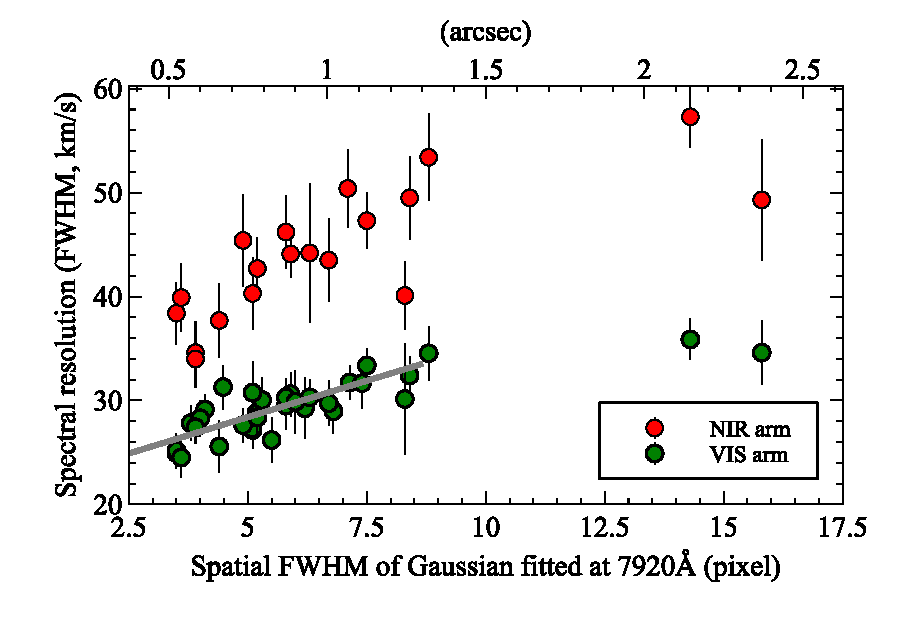
\includegraphics[width=8cm]{figures/resolution_paper.eps}}
		\caption{Green datapoints show the FWHM (km/s) of Gaussian fits to unresolved telluric absorption lines in the VIS spectra, as a function of the FWHM of a Gaussian fit onto the trace in spatial direction at  792 nm. The lower horizontal axis is in units pixels, the top axis in arc seconds. The red datapoints show a subsample of NIR spectra.
			The grey line shows a linear fit to the VIS datapoints. }
		\label{fig:res}
	\end{figure}
	
	\subsection{Correction for offsets in the wavelength calibration}    
	
	X-shooter, being installed at the VLT Cassegrain focusi is  prone to
	flexures during operations. The flexures modify the projection of the slit
	on the detector with respect to the one obtained in daytime calibration. 
	This require a modification of the wavelength solution in order to
	process correctly the night-time data. Part of this correction
	is performed by the pipeline using the frames taken
	during X-shooter Active Flexure Compensation procedure
	\footnote{X-shooter User Manual available at https://www.eso.org/sci/facilities/paranal/instruments/xshooter/doc.html}
	We corrected the remaining part using as a reference the sky
	emission lines present in the observed data.
	
	
	For every afterglow observation we reduced one frame individually in STARE mode without
	sky subtraction obtaining $\sim$ 100 sky spectra. The sky line list compiled at ESO for
	the E-ELT
	study\footnote{http://www.eso.org/sci/facilities/eelt/science/drm/tech\_data/data/optical\_ir\_sky\_lines.dat}
	from the work of (Hanuschik, 2003, A\&A, 407, 1157) and (Rousselot et al. (2000, A\&A, 354, 1134), was used as a reference.
	From this list, we selected a subset of bright and isolated lines. In the case of the OH doublets, unresolved at X-shooter resolution, we took as line position the average between the blue and red components. To find the offsets of the spectra, we fitted gaussians near the
	expected positions under IDL using the MPFIT software (Markwardt, 2009, Astronomical Society of the Pacific Conference Series, Vol. 411, ADASS XVII, ed. D.A. Bohlender, D. Durand, \& P. Dowler, 251) and we compared the result to the tabulated values.
	The resulting offsets, which were smaller than 0.1 \AA~in the UVB and VIS data
	and smaller than 0.5 \AA~in the NIR spectra, were applied to the corresponding spectra.

	
	\section{Results}
	\LongTables
	
	\begin{deluxetable*}{@{\extracolsep{\fill}}lcccccclc@{}}
		%\tabletypesize{\scriptsize}
		%\rotate
		\tablecaption{The full sample of afterglows or hosts observed in the program.
			We here list the burst names and details of the spectroscopic observations. The
			exposure times and slit widths are given in the order UVB/VIS/NIR. The column
			$\Delta t$ shows the time after trigger when the spectroscopic observation was
			started. Mag$_\mathrm{acq}$ gives the approximate magnitude (typically in the
			$R$-band) of the afterglow in the acquisition image.
			\label{sample}}
		\tablewidth{0pt}
		\tablehead{
			\colhead{GRB} &  \colhead{Exptime} & \colhead{Slit width} & \colhead{Airmass} & \colhead{Seeing} & \colhead{$\Delta t$} & \colhead{Mag$_\mathrm{acq}$} & \colhead{Redshift} & \colhead{Ref}\\
			&  \colhead{(ks)}   & \colhead{(arcsec)} &   & \colhead{(arcsec)} & \colhead{(hr)}       &  & &  \\
		}
		\startdata
		GRB090313$^1$ 		& 6.9/6.9/6.9     	& 1.0/0.9/0.9 		& 1.2--1.4  	& 1.0  	&    45  	&  21.6  	& 3.3736 		& (1) \\
		GRB090530$^1$ 		& 4.8/4.8/4.8     	& 1.0/1.2/1.2 		& 1.6--2.2  	& 1.5  	&    20  	&  22    	& 1.266 		& (2) \\
		GRB090809$^1$ 		& 7.2/7.2/7.2     	& 1.0/0.9/0.9 		& 1.2--1.1  	& 0.9  	&  10.2  	&  21    	& 2.737  		& (2,3) \\
		GRB090926$^1$ 		& 7.2/7.2/7.2     	& 1.0/0.9/0.9 		& 1.4--1.5  	& 0.9  	&    22  	&  17.9  	& 2.1062 		& (4) \\
		GRB091018     		& 2.4/2.4/2.4     	& 1.0/0.9/0.9 		& 2.1--1.8  	& 0.8  	&   3.5  	&  19.1  	& 0.9710 		& (5) \\  
		GRB091127     		& 6.0/6.0/6.0     	& 1.0/0.9/0.9 		& 1.1--1.2  	& 1.0  	&   101  	&  21.2  	& 0.490  		& (6) \\
		GRB100205A     		& 10.8/10.8/10.8 	& 1.0/0.9/0.9 		& 1.9--1.8  	& 1.0  	&    71  	&   --   	&  --    		& (2) \\
		GRB100219A     		&  4.8/4.8/4.8   	& 1.0/0.9/0.9 		& 1.3--1.1  	& 0.7  	&  12.5  	&   23   	& 4.667  		& (7) \\
		GRB100316B     		&  2.4/2.4/2.4   	& 1.0/0.9/0.9 		& 2.0--2.4  	& 0.7  	&   0.7  	&  18.2  	& 1.18   		& (2) \\
		GRB100316D-1$^2$ 	&  7.2/7.2/7.2   	& 1.0/0.9/0.9 		& 1.2--1.5  	& 1.0  	&  12  		&   --   	& 0.059  		& (8) \\
		GRB100316D-2   		&  2.4/2.4/2.4   	& 1.0/0.9/0.9 		& 1.2--1.2  	& 1.0  	&    58  	&   --   	& 0.059  		& (8) \\
		GRB100316D-3   		&  2.4/2.4/2.4   	& 1.0/0.9/0.9 		& 1.2--1.2  	& 0.8  	&   192  	&   --   	& 0.059  		& (8) \\
		GRB100418A-1   		&  4.8/4.8/4.8   	& 1.0/0.9/0.9 		& 1.6--1.3  	& 0.7  	&   8.4  	&  18.1  	& 0.6235 		& (9) \\
		GRB100418A-2   		&  4.8/4.8/4.8   	& 1.0/0.9/0.9 		& 1.2--1.3  	& 0.6  	&    34  	&  19.2   	& 0.6235 		& (9) \\
		GRB100418A-3   		&  4.8/4.8/4.8   	& 1.0/0.9/0.9 		& 1.2--1.4  	& 0.7  	&    58  	&   --   	& 0.6235 		& (9) \\
		GRB100424A$^3$ 		&  4.8/4.8/4.8   	& 1.0/0.9/0.9 		& 1.1--1.2  	& 0.8  	&   --   	&   --   	& 2.465  		& (2) \\
		GRB100425A     		&  2.4/2.4/2.4   	& 1.0/0.9/0.9 		& 1.5--1.3  	& 0.7  	&   4.0  	&  20.6  	& 1.755  		& (2,3) \\
		GRB100621A     		&  2.4/2.4/2.4   	& 1.0/0.9/0.9 		& 1.3--1.4  	& 1.0  	&   7.1  	&   --   	& 0.542  		& (2) \\
		GRB100625A$^3$ 		&  4.8/4.8/4.8   	& 1.0/0.9/0.9 		& 1.1--1.0  	& 0.8  	&    13  	&   --   	& 0.452  		& (2) \\
		GRB100724A$^4$ 		&  4.2/4.2/4.2   	& 1.0/0.9/0.9 		& 1.5--2.3  	& 0.7  	&   0.2  	&   --   	& 1.288  		& (2) \\
		GRB100728B$^5$ 		&  7.2/7.2/7.2   	& 1.0/0.9/0.9 		& 1.5--1.1  	& 0.5  	&    22  	&   23   	& 2.106  		& (2) \\
		GRB100814A-1$^4$ 	& 0.9/0.9/0.9  		& 1.0/0.9/0.9 		& 1.9--1.7  	& 0.5  	&   0.8  	&   19   	& 1.44   		& (2) \\
		GRB100814A-2   		&  4.8/4.8/4.8   	& 1.0/0.9/0.9 		& 1.5--1.2  	& 0.6  	&   1.4  	&   19   	& 1.44   		& (2) \\
		GRB100814A-3   		&  4.8/4.8/4.8   	& 1.0/0.9/0.9 		& 1.2--1.0  	& 0.6  	&   99   	&   20   	& 1.44   		& (2) \\
		GRB100816A$^6$ 		&  4.8/4.8/4.8   	& 1.0/0.9/0.9 		& 1.8--1.6  	& 0.8  	&   3.7  	&   --   	& 0.806  		& (2) \\
		GRB100901A     		&  2.4/2.4/2.4   	& 1.0/0.9/0.9 		& 1.5--1.5  	& 1.8  	&   66   	&   --   	& 1.408  		& (10) \\
		GRB101219A     		&  7.2/7.2/7.2   	& 1.0/0.9/0.9 		& 1.1--1.7  	& 2.0  	&   3.7  	&   --   	& 0.718  		& (2) \\
		GRB101219B-1   		&  4.8/4.8/4.8   	& 1.0/0.9/0.9 		& 1.6--2.6  	& 1.3  	&  11.6  	&   20   	& 0.5519 		& (11) \\
		GRB101219B-2   		&  7.2/7.2/7.2   	& 1.0/0.9/0.9 		& 1.2--2.0  	& 0.8  	&   394  	&  22.7  	& 0.5519 		& (11) \\
		GRB101219B-3   		&  7.2/7.2/7.2   	& 1.0/0.9/0.9 		& 1.4--2.1  	& 0.9  	&   886  	&   --   	& 0.5519 		& (11) \\
		GRB110128A     		&  7.2/7.2/7.2   	& 1.0/0.9/0.9 		& 2.0--1.6  	& 0.9  	&   5.5  	&  22.5  	& 2.339  		& (2) \\
		GRB110407A     		&  9.6/9.6/9.6   	& 1.0/0.9/0.9 		& 1.4--1.3  	& 2.0  	&  12.4  	&   23   	&  --    		& (2) \\
		GRB110709B$^1,3$ 	&  7.2/7.2/7.2 		& 1.0/0.9/0.9 		& 1.6--1.1  	& 1.0  	&   --   	&   --   	&  --    		& (2) \\
		GRB110715A     		&  0.6/0.6/0.6   	& 1.0/0.9/0.9 		& 1.1--1.1  	& 1.7  	&  12.3  	&  18.5  	& 0.82  		& (2) \\
		GRB%110721A     	&  2.4/2.4/2.4   	& 1.0/0.9/0.9 		& 1.2--1.4  	& 2.4  	&        	&        	& 0.382  		& (2) \\
		GRB110808A     		& 2.4/2.4/2.4    	& 1.0/0.9/0.9 		& 1.2--1.1  	& 1.1  	&   3.0  	&  21.2  	& 1.3488 		& (2) \\
		GRB110818A     		& 4.8/4.8/4.8    	& 1.0/0.9/0.9 		& 1.3--1.3  	& 1.0  	&   6.2  	&  22.3  	& 3.36   		& (2) \\
		GRB111005A$^3$ 		& 1.2/1.2/1.2    	& 1.0/0.9/0.9 		& 1.3--1.3  	& 0.7  	&   --   	&  --    	& 0.013? 		& (2) \\
		GRB111008A-1   		& 8.8/8.8/8.4    	& 1.0/0.9/0.9 		& 1.1--1.0  	& 1.2  	&   8.5  	&  21?   	& 4.9898 		& (12) \\
		GRB111008A-2   		& 8.0/8.0/7.2    	& 1.0/0.9/0.9 		& 1.3--1.0  	& 1.0  	&  20.1  	&  22?   	& 4.9898 		& (12) \\
		GRB111107A     		& 4.8/4.8/4.8    	& 1.0/0.9/0.9 		& 1.8--1.5  	& 0.7  	&   5.3  	&  21.5  	& 2.893  		& (2) \\
		GRB111117A$^6$ 		& 4.8/4.8/4.8    	& 1.0/0.9/0.9 		& 1.5--1.4  	& 0.6  	&    38  	&  --    	& 1.3?   		& (2) \\
		GRB111123A-1   		& 6.2/6.6/6.6    	& 1.0/0.9/0.9 		& 1.6--1.1  	& 1.0  	&  12.2  	&  $>$24 	& 3.1516 		& (2) \\
		GRB111123A-2$^3$ 	& 2.4/2.4/2.4  		& 1.0/0.9/0.9 		& 1.0--1.0  	& 0.5  	&   --   	&  --    	& 3.1516 		& (2) \\
		GRB111129A     		& 3.6/3.6/3.6    	& 1.0/0.9/0.9 		& 1.6--2.1  	& 1.7  	&        	&        	&  --    		& (2) \\
		GRB111209A-1   		& 4.8/4.8/4.8    	& 1.0/0.9/0.9 		& 1.1--1.2  	& 0.8  	&  17.7  	&  20.1  	& 0.677  		& (13) \\
		GRB111209A-2   		& 9.6/9.6/9.6    	& 1.0/0.9/0.9 		& 1.2--2.0  	& 0.8  	&  497   	&  23    	& 0.677  		& (13) \\
		GRB111211A$^1$ 		& 2.4/2.4/2.4    	& 1.0/0.9/0.9 		& 1.4--1.6  	& 0.6  	&   31   	&  19.5  	& 0.478  		& (2) \\
		GRB111228A     		& 2.4/2.4/2.4    	& 1.0/0.9/0.9 		& 1.4--1.4  	& 0.9  	&  15.9  	&  20.1  	& 0.716  		& (2) \\
		GRB120118B$^3$ 		& 3.6/3.6/3.6    	& 1.0/0.9/0.9 		& 1.1--1.0  	& 1.0  	&   --   	&  --    	& 2.943  		& (2) \\
		GRB120119A-1   		& 2.4/2.4/2.4    	& 1.0/0.9/0.9 		& 1.1--1.1  	& 0.6  	&   1.4  	&   17   	& 1.728  		& (2) \\
		GRB120119A-2   		& 1.2/1.2/1.2    	& 1.0/0.9/0.9 		& 1.8--1.9  	& 0.6  	&   4.5  	&   20   	& 1.728  		& (2) \\
		GRB120119A-3$^3$ 	& 4.8/4.8/4.8  		& 1.0/0.9/0.6JH 	& 1.0--1.1  	& 1.1 	&   --   	&   --   	& 1.728  		& (2) \\
		GRB120211      		&                	&             		&           	&      	&        	&         	& 2.346 		& (2) \\
		GRB120224A     		& 2.4/2.4/2.4    	& 1.0/0.9/0.9 		& 1.7--2.1  	& 1.4  	&  19.8  	&   22.3 	&  --    		& (2) \\
		GRB120311A     		& 2.4/2.4/2.4    	& 1.0/0.9/0.9 		& 1.6--1.4  	& 0.6  	&   3.7  	&   21.6 	&  --    		& (2) \\
		GRB120327A-1   		& 2.4/2.4/2.4    	& 1.0/0.9/0.9 		& 1.6--1.4  	& 0.5  	&   2.1  	&   18.8 	& 2.815  		& (14) \\
		GRB120327A-2   		& 4.2/4.2/4.2    	& 1.0/0.9/0.9 		& 1.0--1.1  	& 1.0  	&    29  	&   22.5 	& 2.815  		& (14) \\
		GRB120404A     		& 9.6/9.6/9.6    	& 1.0/0.9/0.9JH 	& 1.7--1.3 		& 1.3 	&  15.7  	&   21.3 	& 2.876  		& (2) \\
		GRB120422A-1   		& 4.8/4.8/4.8    	& 1.0/0.9/0.9 		& 1.3--1.3  	& 0.6  	&  17.2  	&   22.0 	& 0.283  		& (15) \\
		GRB120422A-2   		& 4.8/4.8/4.8    	& 1.0/0.9/0.9 		& 1.3--1.4  	& 0.9  	&  113   	&   --   	& 0.283  		& (15) \\
		GRB120422A-3   		& 4.8/4.8/4.8    	& 1.0/0.9/0.9 		& 1.4--1.7  	& 1.0  	&  210   	&   --   	& 0.283  		& (15) \\
		GRB120422A-4   		& 4.8/4.8/4.8    	& 1.0/0.9/0.9JH 	& 1.3--1.4 		& 0.6  	& 449   	&   --   	& 0.283  		& (15) \\
		GRB120422A-5   		& 4.8/4.8/4.8    	& 1.0/0.9/0.9JH 	& 1.3--1.6 		& 0.8  	& 593   	&   --   	& 0.283  		& (15) \\
		GRB120422A-6   		& 4.8/4.8/4.8    	& 1.0/0.9/0.9JH 	& 1.7--2.4 		& 2.5  	& 882   	&   --   	& 0.283  		& (15) \\
		GRB120422A-7   		& 4.8/4.8/4.8    	& 1.0/0.9/0.9JH 	& 1.5--1.9 		& 1.3  	& 906   	&   --   	& 0.283  		& (15) \\
		GRB120712A     		& 4.8/4.8/4.8    	& 1.0/0.9/0.9   	& 1.5--2.5 		& 1.3  	& 10.4  	&   21.5 	& 4.175  		& (2) \\
		GRB120714B     		& 4.8/4.8/4.8    	& 1.0/0.9/0.9JH 	& 1.5--1.2 		& 1.2  	&  7.8  	&   22.1 	& 0.398  		& (2)\\
		GRB120716A$^1$ 		& 3.6/3.6/3.6    	& 1.0/0.9/0.9JH 	& 1.8--2.6 		& 1.0  	&  62   	&   20.9 	& 2.486  		& (2) \\
		GRB120722A$^2$ 		& 4.8/4.8/4.8    	& 1.0/0.9/0.9   	& 1.3--1.3 		& 1.1  	& 10.3  	&   23.6 	& 0.959  		& (2) \\
		GRB120805A$^2$ 		& 3.6/3.6/3.6    	& 1.0/0.9/0.9JH 	& 1.3--1.7 		& 0.9  	& 218   	&   --   	& 2.8?   		& (2) \\
		GRB120815A     		& 2.4/2.4/2.4    	& 1.0/0.9/0.9   	& 1.3--1.4 		& 0.6  	&  1.7  	&   20   	& 2.358  		& (16) \\
		GRB120909A     		& 1.2/1.2/1.2    	& 1.0/0.9/0.9   	& 1.6--1.6 		& 1.4  	&  1.7  	&   21   	& 3.929  		& (2) \\
		GRB120923A     		& 9.6/9.6/9.6    	& 1.0/0.9/0.9JH 	& 1.2--1.4 		& 1.0  	& 18.5  	&   --   	& $\gtrsim8$ 	& (2) \\
		GRB121024A     		& 2.4/2.4/2.4    	& 1.0/0.9/0.9   	& 1.2--1.1 		& 0.6  	&  1.8  	&   20   	& 2.300  		& (17) \\
		GRB121027A     		& 8.4/8.4/8.4    	& 1.0/0.9/0.9   	& 1.3--1.3 		& 0.9  	&  69   	&  21.1  	& 1.773  		& (2) \\
		GRB121201A     		& 4.8/4.8/4.8    	& 1.0/0.9/0.9JH 	& 1.1--1.1 		& 0.9  	& 12.9  	&   23   	& 3.385  		& (2) \\
		GRB121229A     		& 4.8/4.8/4.8    	& 1.0/0.9/0.9JH 	& 1.4--1.2 		& 1.4  	&  2.0  	&  21.5  	& 2.707  		& (2) \\
		GRB130131B$^3$ 		& 7.2/7.2/7.2    	& 1.0/0.9/0.9JH 	& 1.3--1.6 		& 0.8  	&  --   	&   --   	& 2.539  		& (2) \\
		GRB130408A     		& 1.2/1.2/1.2    	& 1.0/0.9/0.9   	& 1.0--1.0 		& 1.0  	&  1.9  	&   20   	& 3.758  		& (2) \\
		GRB130418A     		& 1.2/1.2/1.2    	& 1.0/0.9/0.9   	& 1.4--1.3 		& 1.3  	&  4.6  	&   18.5 	& 1.218  		& (2) \\
		GRB130427A     		& 1.2/1.2/1.2    	& 1.0/0.9/0.9JH 	& 1.8--1.8 		& 0.8  	& 16.5  	&   19   	& 0.340  		& (18) \\
		GRB130427B     		& 1.2/1.2/1.2    	& 1.0/0.9/0.9JH 	& 1.2--1.0 		& 0.8  	& 20.3  	&   22.7 	& 2.78   		&  (2) \\
		GRB130603B$^6$ 		& 2.4/2.4/2.4    	& 1.0/0.9/0.9   	& 1.4--1.4 		& 1.1  	&  8.2  	&   21.5 	& 0.356  		& (19) \\
		GRB130606A     		& 4.2/4.2/4.2    	& 1.0/0.9/0.9JH 	& 1.7--1.9 		& 1.1  	&  7.1  	&   19   	& 5.91   		& (20) \\
		GRB130612A     		& 1.2/1.2/1.2    	& 1.0/0.9/0.9   	& 1.3--1.3 		& 1.4  	&  1.1  	&   21.5 	& 2.006  		& (2) \\
		GRB130615A     		& 1.2/1.2/1.2    	& 1.0/0.9/0.9   	& 2.1--2.2 		& 1.0  	&  0.8  	&   21   	& $~3$?  		& (2) \\
		GRB130701A     		& 1.2/1.2/1.2    	& 1.0/0.9/0.9JH 	& 2.0--2.0 		& 1.6  	&  5.5  	&   19.9 	& 1.155  		& (2) \\
		\enddata
		\tablenotetext{1}{Not part of the statistical sample}
		\tablenotetext{2}{Spectrum dominated by light from the host galaxy}
		\tablenotetext{3}{Spectrum of the host galaxy taken long after the burst}
		\tablenotetext{4}{RRM observation}
		\tablenotetext{5}{ADC malfunction during observation}
		\tablenotetext{6}{Short burst}
		\tablerefs{
			(1) \citet{DeUgartePostigo2010}; (2) This work ; (3) Skuladottir (2010);
			(4) \citet{DElia2010}; (5) \citet{Wiersema2012}; (6) \citet{Vergani2011, Cobb2010}; 
			(7) \citet{Thone2013}; (8) \citet{Bufano2012} ; (9) \citet{DeUgartePostigo2011} ;
			(10) \citet{Hartoog2013}; (11) \citet{Sparre2011}; (12) \citet{Sparre2014};
			(13) \citet{Levan2014}; (14) \citet{DElia2014}; (15) \citet{Schulze2014};
			(16) \citet{Kruhler2013}; (17} \citet{Friis2015}
	\end{deluxetable*}
	%-------------------------END TABLE---------------------------------------
		
	
	\subsection{Complete sample}	
	
	
	\subsection{Follow-up timing and afterglow brightness}
	This sections should contain a plot og the follow-up delay and the acquisition image brightness at the time of observations. 
	
	\subsection{Properties of rejected triggers}
	How many bursts have been excluded due to particularities in the follow-up attempt. Visitor, Weather, technical issues.  	
	
	\subsection{On the nature of triggered GRBs without detected optical afterglow.}
	This should include observations where the acquisition image has been taken, but observations were discontinued due to non-detection. What are the X-ray properties of these bursts?
	
	
	\subsection{Redshifts}
	
	\subsubsection{Afterglow-based redshifts}
	
	\subsubsection{Emissionline-based redshifts}	
	Redshift completeness
	
	\subsection{Hydrogen column densities}
	
	\subsubsection{Comparison to X-ray determined columns}	

	
	\section{Discussion}
	
	\subsection{Comparison to previous samples.}	
	This should also include a discussion of dark bursts. 
	Cuchiara. BAT6 (Salvaterra), TOUGH
	
		
	\subsection{Comparison to previous samples.}		
	
	
	\subsection{X-ray column densities vs. optically derived ones}	
		
	\subsection{Why is the HI column truncated?}
	
	What is the expected transmission for a high-column HI, where the hydrogen primarily will be in the form of H2? 
	
	
	
	
	\section{Conclusion}
	
	
	\begin{acknowledgements}
		JPUF, BMJ and DX acknowledge support from the ERC-StG grant EGGS-278202.  The
		Dark Cosmology Centre is funded by the Danish National Research Foundation.  TK
		acknowledges support by the European Commission under the Marie Curie
		Intra-European Fellowship Programme in FP7.  AdUP acknowledges support by the
		European Commission under the Marie Curie Career Integration Grant programme
		(FP7-PEOPLE-2012-CIG 322307).  This work made use of data supplied by the UK
		{\it Swift} Science Data Centre at the University of Leicester.  Finally, we
		acknowledge expert support from the ESO staff at the Paranal and La Silla
		observatories in obtaining these target of opportunity data.
		
	\end{acknowledgements}
	
	\def\aj{AJ}
	\def\araa{ARA\&A}
	\def\apj{ApJ}
	\def\apjl{ApJL}
	\def\apjs{ApJS}
	\def\apss{Ap\&SS}
	\def\aap{A\&A}
	\def\aapr{A\&A~Rev.}
	\def\aaps{A\&AS}
	\def\mnras{MNRAS}
	\def\nat{Nature}
	\def\pasp{PASP}
	\def\aplett{Astrophys.~Lett.}
	
	\bibliographystyle{apj}
	\bibliography{XSGRB_sample}
	%\bibliography{thebib}
	
	
	\newpage
	\appendix

	\section{Notes on Individual objects}
	
	\subsection{GRB090313}
	
	\subsection{GRB100205A}
	Observed 3 days after the \textit{Swift} trigger. No afterglow or host detected
	in 10.8 ks. GRB likely located at high
	redshift\footnote{\url{http://gcn.gsfc.nasa.gov/gcn3/10399.gcn3}}. The spectrum
	has not otherwise been published previously.
	
	\subsection{GRB100219A (z = 4.667)}
	The data presented here also formed the basis of GCN \#
	10441\footnote{\url{http://gcn.gsfc.nasa.gov/gcn3/10441.gcn3}} and is published
	in \citet{Thone2013}. Observations started 12.5 hours after the \textit{Swift}
	trigger and has a total exposure time of 4.8 ks. Absorption features, including
	those of \lya, from a multitude of ions are detected against the afterglow
	continuum at $z = 4.667$. Additionally, absorption from an intervening system
	is found at $z = 2.181$.
	
	\subsection{GRB100316B (z = 1.180)}
	The data presented here also formed the basis of GCN \#
	10495\footnote{\url{http://gcn.gsfc.nasa.gov/gcn3/10495.gcn3}}. The spectrum
	has not otherwise been published previously. Observations started 44 minutes
	after the \textit{Swift} trigger and has a total exposure time of 2.4 ks.
	Absorption features from \feii, \alii, \aliii,	\mgii~and \mgi~are well detected
	against the afterglow continuum at $z = 1.180$. Additionally, strong absorption
	lines from \feii~and \mgii~from an intervening system are found at $z = 1.063$.
	
	\subsection{GRB100316D (z = 0.059)}
	The data presented here also formed the basis of GCN \#
	10512\footnote{\url{http://gcn.gsfc.nasa.gov/gcn3/10512.gcn3}}, GCN \#
	10513\footnote{\url{http://gcn.gsfc.nasa.gov/gcn3/10513.gcn3}}, GCN \#
	10543\footnote{\url{http://gcn.gsfc.nasa.gov/gcn3/10543.gcn3}} and is published
	in \citet{Bufano2012} and \citet{Starling2011}. This GRB is very close by and
	has an associated SN, SN2010bh, and has therefore undergone intense follow-up. The data
	presented here consists of a subset of the entire VLT/X-shooter campaign,
	covering the four first observing days while the afterglow still contributes
	significantly to the total emission. The first observations started 10 hours
	after the burst, before the SN was discovered, and targeted the star-forming
	'A'-region\citep{Starling2011}, not the GRB. A very rich spectrum containing a
	multitude of emission lines puts the host at $z = 0.059$. For three consequtive
	nights, 58, 79 and 101 hours after the \textit{Swift} trigger, the afterglow
	was observed as it transitioned into the spectrum of a high-velocity Ic-BL SN.
	The observations taken 79 and 101 hours after the burst are taken under
	programme 084.D-0265(A) (PI: Benetti), but with an identical setup to the first
	two observations.
	
	\subsection{GRB100418A (z=0.624)}
	The data presented here also formed the basis of GCN \#
	10620\footnote{\url{http://gcn.gsfc.nasa.gov/gcn3/10620.gcn3}} and GCN \#
	10631\footnote{\url{http://gcn.gsfc.nasa.gov/gcn3/10631.gcn3}} and is published
	in \citet{DeUgartePostigo2011}. The burst have been followed up in three epochs
	of observations, 0.4, 1.4, and 2.4 days after the burst, each lasting 4.8 ks.
	The unambiguous redshift of the host, $z=0.624$, is found from the simultaneous
	detection of emission features belonging to nebular lines, including \hi, \oii,
	\oiii, \neiii, \nii, \sii, \siii, and \hei~as well as absorption features due
	to the presence of \znii, \crii, \feii, \mnii, \mgii, \mgi, \tiii, and \caii,
	all at a consistent redshift. Temporal evolution of the fine-structure lines
	belonging to \feii$^*$ is found between the epochs.

	\subsection{GRB100424A (z=2.465)}
	The data presented here also formed the basis of GCN \#
	14291\footnote{\url{http://gcn.gsfc.nasa.gov/gcn3/14291.gcn3}}. The spectrum
	has not otherwise been published previously. Observations carried out, long
	after the burst has faded.  Emission lines from the host are detected at
	$z=2.465$.

	\subsection{GRB100425A (z=1.1755)}
	The data presented here also formed the basis of GCN \#
	10684\footnote{\url{http://gcn.gsfc.nasa.gov/gcn3/10684.gcn3}} and is used in
	\citet{Skuladottir2010}, but not published elsewhere. Observations started 4
	hours after the \textit{Swift} trigger, totaling 2.4 ks. Absorption features
	from \mgii~and \feii~in the afterglow continuum are detected at $z=1.1755$.

	\subsection{GRB100615A (z=1.398)}
	The data presented here also formed the basis of GCN \#
	14264\footnote{\url{http://gcn.gsfc.nasa.gov/gcn3/14264.gcn3}}, but not
	published elsewhere. Host observation of a dark burst\citep{DElia2011} taken
	long after the afterglow has faded. Emission lines from the host belonging to
	\oii, \neiii, \oiii~and \ha~are detected at a common redshift of $z=1.398$.
	
	\subsection{GRB100621A (z=0.542)}
	The data presented here also formed the basis of GCN \#
	10876\footnote{\url{http://gcn.gsfc.nasa.gov/gcn3/10876.gcn3}}, but not
	published elsewhere. Beginning 7.1 hours after the GRB, 2.4 ks observations
	reveal emission lines from \oii, \hb~and \oiii~at a common redshift of
	$z=0.542$ and a very weak afterglow continuum.

	\subsection{GRB100625A (z=0.452)}
	The data presented here is of the candidate host galaxy, taken long after the
	burst has faded and have not previously been published. 4.8 ks of exposure
	reveals a weak continuum present in all arms, but an absence of emission lines.
	This could indicate that the host primarily contains a older stellar
	population. The redshift, $z=0.452$, is taken from \citet{Fong2013}.

	
	\subsection{GRB100724A* (z = 1.288)}
	The data presented here also formed the basis of GCN \#
	10971\footnote{\url{http://gcn.gsfc.nasa.gov/gcn3/10971.gcn3}}. The spectrum
	has not otherwise been published previously. The observations were carried out
	in RRM starting 11 min after the GRB trigger. See section \ref{RRM}, for a
	description of the RRM scheme. Absorption lines from several ionic species are
	detected in the afterglow continuum at a common redshift of $z = 1.288$. This
	is not a part of the statistical sample.

	\subsection{GRB100728B (z=2.106)}
	The data presented here also formed the basis of GCN \#
	11317\footnote{\url{http://gcn.gsfc.nasa.gov/gcn3/11317.gcn3}}. The spectrum
	has not otherwise been published previously. Starting 22 hours after the burst
	trigger, 7.2 ks of observations reveals a faint afterglow continuum with \lya-
	and \mgii-absorption at $z=2.106$. Due to a malfunctioning ADC, the sensitivity
	of X-shooter is depressed with respect to normal operations, resulting in a
	poorer throughout. Additionally, the position of the trace on the slit moves
	due to atmospheric differential refraction.

	\subsection{GRB100814A (z=1.439)}
    The spectra presented here has not been published previously. The
    observations consists of three visits, the first beginning only 0.9 hours
    after the \textit{Swift} trigger, the other two visits were 2.13 and 98.40
    hours after the trigger, respectively. A bright afterglow continuum is
    present in all visits, allowing identification of absorption features
    belonging to a wide range of ions at $z=1.439$. A complex velocity structure
    in the absorption features belonging to \mgii, shows several components,
    separated by as much as 500km/s, pointing to a likely merger scenario in
    the host.
    
	\subsection{GRB100816A (z=0.805)}
	The data presented here also formed the basis of GCN \#
	11123\footnote{\url{http://gcn.gsfc.nasa.gov/gcn3/11123.gcn3}}. The spectrum
	has not otherwise been published previously. This short GRB was observed 28.4
	hours after the GRB trigger. 4 x 1200 s of exposure reveals two distinct sets
	of emission lines, spatially offset $\lesssim 1 \arcsec $, very close in
	redshift space, $z=0.8034$ and $z=0.8049$, indicating either an interacting
	host or some complex velocity structure of the host. Faint underlying continua
	are present under both sets of lines.

	\subsection{GRB100901A (z=1.408)}
	The data presented here has been published in \citet{Hartoog2013}. Because of
	the unusual lingering brightness of this GRB, 2.4s of observations taken 65.98
	hours after the GRB trigger still reveals an afterglow continuum visible across
	the entire spectral coverage of X-shooter. Absorption lines from a wide range
	ion put the redshift at $z=1.408$, with intervening absorption systems at $z =
	1.3147$ and $z = 1.3179$.

	\subsection{GRB101219A (z=0.718)}
	This data has not been published before. Starting 3.7 hours after the GRB
	trigger, 7.2 ks of exposure time reveals a very faint continuum in the visual
	and near-infrared, only visible when heavily binning the images. No redshift
	estimate is available from these observations.  Late-time Gemini-North
	observations reveal emission lines from the host at
	$z=0.718$\footnote{\url{http://gcn.gsfc.nasa.gov/gcn3/11518.gcn3}}.

	\subsection{GRB101219B (z=0.552)}
	The data presented here also formed the basis of GCN \#
	11579\footnote{\url{http://gcn.gsfc.nasa.gov/gcn3/11579.gcn3}} and is published
	in \citet{Sparre2011}.	The first observation, taken 11.6 hours after the burst
	trigger and lasting 4.8ks, reveals absorption from \mgii~and \mgi~in the host
	located at $z = 0.552$ on a featureless continuum visible across the entire
	coverage of X-shooter.  Subsequent observations taken 16 and 37 days after the
	trigger shows the fading spectral signature of a SN, SN2010ma.

	\subsection{GRB120118B (z = 2.943)}
	The data presented here also formed the basis of GCN \#
	14225\footnote{\url{http://gcn.gsfc.nasa.gov/gcn3/14225.gcn3}}, but is not
	published otherwise. This late-time observation of the host of GRB120118B
	consists of 3.6 ks exposures and contains emission lines belonging to \oii and
	\oiii at $z =	2.943$, suggested to be redshift of the host.

	\subsection{GRB120119A (z = 1.728)}
	The data presented here has not been published before. Three epochs of
	observations have been obtained, the first two immediately after the burst, and
	the last one long after the afterglow had faded. Starting 1.4 hours after the
	\textit{Swift} trigger, the first epoch contains bright afterglow continuum.
	Rich in absorption features belonging to a multitude of ions, $z =	1.728$ is
	estimated for the host with intervening systems at $z =	1.476$, $z = 1.214$, $z
	= 0.662$ and $z = 0.632$. The second epoch, obtained 4.5 hours after the burst
	contains the fading afterglow. A third epoch is obtained $>1$ year after the
	GRB in which emission lines from \hb~and \ha~are found at the redshift of the
	host, confirming the association of the absorption line system and the host.
	
	\subsection{GRB120211A (z = 2.346)}
	The data presented here has been published in \citet{Kruhler2015}. Two
	observations of the host of GRB120211A has been obtained, starting 2013.02.17,
	$> 1 year$ after the burst has faded. A redshift for this object has been
	reported by \citet{Kruhler2015} and the features seen by those authors are
	reproduced in these reductions, confirming $z =	2.346$.

	\subsection{GRB120224A (z = 1.10 NEW!!!)}
	The data presented here has formed the basis of GCN \#
	12991\footnote{\url{http://gcn.gsfc.nasa.gov/gcn3/12991.gcn3}}, and has also
	been published in \citet{Kruhler2015}. Starting 19.8 hours after the GRB
	trigger, a total exposure time of 2.4 ks reveals a faint continuum, starting at
	$\sim$ 7000 \AA~and extending all the way through 25000 \AA. We detect a $\sim
	2 \sigma$ emission line which, if interpreted as \ha, gives $z = 1.10$,
	supporting the redshift reported by \citet{Kruhler2015}.

	\subsection{GRB120311 (z = 0.350 NEW!!!)}
	The data presented here has formed the basis of GCN \#
	12991\footnote{\url{http://gcn.gsfc.nasa.gov/gcn3/12991.gcn3}}, but is not
	published otherwise. Starting just before twilight, 3.65 hours after the burst,
	a faint afterglow continuum is detected at all wavelengths. Due to the
	faintness of the afterglow, no absorption features are discernible superposed
	on the continuum. Displaced from the afterglow continuum by 1\farc4, emission
	lines belonging to \hb, \oiii~and \ha~are detected at $z = 0.350$. The line
	belonging to \ha~shows some extended emission toward the afterglow continuum.
	The angular distance between the two sources correspond to a projected distance
	in the host plane of 6 kpc, posing a potential problem for the host redshift,
	unless the GRB ocurred in a merging system. The extended emission in \ha,
	supports this interpretation. This burst is not apart of the statistical sample.

	\subsection{GRB120327A (z = 2.813)}
	The data presented here also formed the basis of GCN \#
	13134\footnote{\url{http://gcn.gsfc.nasa.gov/gcn3/13134.gcn3}} and is published
	in \citet{DElia2014}. The observation consists of two visits, 2.13 hrs and
	29.98 hrs after the burst, with an afteglow continuum visible in all arms for
	both visits. We detect absorption features from Ly-limit, \lya, \cii/\cii$^*$,
	\SIii/\SIii$^*$, \ali, \feii ~and \mgii ~are detected at a consistent redshift,
	$z = 2.813$.

	\subsection{GRB120404A (z = 2.876)}
	The data presented here has formed the basis of GCN \#
	13227\footnote{\url{http://gcn.gsfc.nasa.gov/gcn3/13227.gcn3}}, but is not
	published otherwise. 9.6 ks integration, starting 15.7 hours after the
	\textit{Swift}-trigger reveals a low-intensity afterglow continuum on which
	absorption from \lya is detected in two distinct regions at redshifts $z=2.876$
	and $z=.255$. These absorption systems are confirmed by ionic absorption
	features at both of these redshifts.

	
	\subsection{GRB120422A (z = 0.283)}
	The data presented here also formed the basis of GCN \#
	13257\footnote{\url{http://gcn.gsfc.nasa.gov/gcn3/13257.gcn3}} and is published
	in \citet{Schulze2014}. A GRB-SN, this burst has been followed up multiple
	times. The data presented here only contain the first epoch in which the
	afterglow is still visible and before the rise of SN2012bz. Starting 16.5 hours
	after the burst, 4.8 ks integration time captures both the host and the burst
	in emission. A blue afterglow continuum is detected at all wavelengths covered
	by X-shooter, on which \mgii absorption at $z = 0.283$ is found. Offset by
	1\farc75, the host is clearly detected at a consistent redshift with a rich
	emission line spectrum, the lines extending towards to burst.

	\subsection{GRB120712A (z = 4.175)}
	The data presented here also formed the basis of GCN \#
	13460\footnote{\url{http://gcn.gsfc.nasa.gov/gcn3/13460.gcn3}} and is not
	published elsewhere. 4.8 ks integration time, starting 10.5 hours after the BAT
	trigger, shows a bright afterglow continuum starting at $\sim$ 4720 \AA,
	signifying the onset of the Lyman alpha forest, for a GRB located at $z =
	4.175$. Absorption features from \lya, \feii, \mgii~and \SIii~are readily
	detected at a consistent redshift.

	\subsection{GRB120714B (z = 0.398)}
	The data presented here also formed the basis of GCN \#
	13477\footnote{\url{http://gcn.gsfc.nasa.gov/gcn3/13477.gcn3}}, but is not
	published elsewhere. Observations of this burst started 7.8 hours after the GRB
	trigger, lasting 4.8 ks. A continuum is visible across the entire spectral
	coverage of X-shooter, with both emission lines from  \oii, \hb, \oiii~and \ha,
	as well as absorption from \mgii~detected at $z = 0.398$, securely setting it
	as the redshift of the GRB.
	
	
	\subsection{GRB120716A (z = 2.486)}
	The data presented here also formed the basis of GCN \#
	13494\footnote{\url{http://gcn.gsfc.nasa.gov/gcn3/13494.gcn3}}, but is not
	published elsewhere. Despite observations starting 62 hours after the
	\textit{Swift} trigger and lasting 3.6 ks, a bright afterglow is clearly seen,
	along with a plethora of absorption features. Absorption of \lya-photons in the
	host leaves a broad trough, from which the Lyman alpha forest is visible
	bluewards, all the way down to the Lyman limit. Metal absorption lines from
	\cii, \SIii, \oi, \feii, \civ, \SIiv, including fine structure transitions
	identified as \cii$^*$, \SIii$^*$, \feii$^*$ and metastable \NIii~lines are all
	detected at $z = 2.486$

	\subsection{GRB120805A (z $\sim$ 3.9 NEW!!!)}
	A separate reduction of this burst has been published in \citet{Kruhler2015},
	but not otherwise. Starting 9 days after the burst trigger, this is host
	observation and does not contain any afterglow continuum. In 3.6 ks integration
	time, we detect a faint continuum visible from 4500 \AA~and all the way through
	21000 \AA, in contrast to what is found previously. The continuum from 4500 -
	6000 \AA is detected at very low significance. If the drop at 4500 \AA~is the
	Lyman limit, this fits with Lyman alpha at $\sim$ 6000 \AA, giving $z \sim
	3.9$. The absence of nebular lines if due to \oii~falling in a telluric
	absorption band and the rest being shifted out of the wavelength coverage.

	\subsection{GRB120815A* (z = 2.358)} 
	Not a part of the statistical sample, thisburst also formed the basis of  GCN
	\# 13649\footnote{\url{http://gcn.gsfc.nasa.gov/gcn3/13649.gcn3}} and is
	published in \citet{Kruhler2013}. Observations started 1.69 hours after the BAT
	trigger and consist of 2.4 ks integration. A bright afterglow continuum is
	detected across the entire spectral coverage of X-shooter, with a multitude of
	absorption lines superposed. Absorption features from the host at $z = 2.358$
	include a DLA as well as metal absorption lines from \nv, \sii, \SIii, \oi,
	\civ, \SIiv, \feii, \alii, \aliii, \mnii, \mgii, and \mgi. Additionally
	fine-structure lines from \NIii and \feii are exited local to the GRB.
	Intervening systems are found at $z = 1.539$, $z = 1.693$, and $z = 2.00$.

	\subsection{GRB120722A (z = 0.959)}
	The data presented here also formed the basis of GCN \#
	13507\footnote{\url{http://gcn.gsfc.nasa.gov/gcn3/13507.gcn3}}, but is not
	published elsewhere. On 4.8 ks integration time, starting 10 hours after the
	burst trigger, the simultaneous detection of absorption features belonging to
	\mgii~and \feii~superposed on a blue continuum, and emission lines from \oii,
	\hg, \hb, \oiii~and \ha, all at $z = 0.959$, confidently sets it as the
	redshift of the GRB.

	\subsection{GRB120909A (z = 3.929)}
	The data presented here has formed the basis of GCN \#
	13730\footnote{\url{http://gcn.gsfc.nasa.gov/gcn3/13730.gcn3}}, but is not
	published otherwise. A very rapid follow-up, starting only 1.7 hours after the
	BAT trigger, this 1.2 ks observation captures a very bright afterglow
	continuum, starting at 4500 \AA, signifying the onset of the Lyman limit for a 
	system at $z = 3.929$. Absorption from high-column density hydrogen leaves very
	prominent absorption features in the form of \lya, \lyb, and \lyg, visible in
	the Lyman alpha forest. Metal absorption lines arising from \feii, \NIii,
	\SIii, \sii, \alii, \aliii, \cii, \oi, \civ, and \znii~are all detected along
	with the corresponding fine-structure lines from (\feii$^*$, \SIii$^*$,
	\oi$^*$, \oi$^**$, \cii$^*$), securely anchoring the redshift of the host.

	\subsection{GRB121024A (z = 2.300)}
	The data presented here also formed the basis of GCN \#
	13890\footnote{\url{http://gcn.gsfc.nasa.gov/gcn3/13890.gcn3}} and is published
	in \citet{Friis2015}. Also rapid, starting 1.8 hours after the \textit{Swift}
	trigger, a bright afterglow continuum is visible across all arms. A broad
	absorption feature from Lyman alpha, along with narrow lines from \civ, \SIii,
	\SIiv, \feii, \sii, and \alii, as well as fine-structure lines associated with
	\SIii$^*$ are all detected at $z = 2.300$, securely setting it as the redshift
	of the GRB.

	\subsection{GRB121027A (z = 1.773)}		
	The data presented here has formed the basis of GCN \#
	13930\footnote{\url{http://gcn.gsfc.nasa.gov/gcn3/13930.gcn3}}, but is not
	published otherwise. Starting 69.6 hours after the GRB trigger, that we detect
	the afterglow continuum a so high significance in all arms with 8.4 ks
	integration, testifies to the brightness of this burst. The concurrent
	identification of emission lines from \oiii~and absorption from \civ, \alii,
	\aliii, \mgi, \mgii, and \feii, tightly constrains the redshift of the burst to
	be $(z = 1.773$

    \subsection{GRB130408A (z = 3.758)}
	The data presented here also formed the basis of GCN \#
	14365\footnote{\url{http://gcn.gsfc.nasa.gov/gcn3/14365.gcn3}}. The spectrum
	has not otherwise been published previously. The observations consists of two
	600sec spectra taken 1.9hrs after the burst. We detect absorption features from
	a wide range of ions. We also detect intervening absorption at $z=1.255$ and
	$z=3.248$.
	
	\subsection{GRB130606A (z = 5.913)}
	The data presented here also formed the basis of GCN \#
	14816\footnote{\url{http://gcn.gsfc.nasa.gov/gcn3/14816.gcn3}} and is published
	in \citet{Hartoog2015}. The observations consists of three 2x600sec visits
	starting 7.1 hrs after the burst at fairly high airmass. We detect absorption
	features from a wide range of ions at $z=5.913$ as well as intervening
	absorption at $z=2.3103, 2.5207, 3.4515, 4.4660, 4.5309, 4.5427, 4.6497 $ and $
	4.7244$.

	\subsection{GRB151021A (z = 2.330)}
	The data presented here also formed the basis of GCN \#
	18426\footnote{\url{http://gcn.gsfc.nasa.gov/gcn3/18982.gcn3}} and is not
	published elsewhere. The observation was carried out in RRM starting 44 minutes
	after the GRB trigger. We detect absorption features from a wide range of ions
	at $z=2.330$ as well as intervening absorption at $z=1.49$.

	\subsection{GRB160203A (z = 3.517)}
	The data presented here also formed the basis of GCN \#
	18982\footnote{\url{http://gcn.gsfc.nasa.gov/gcn3/18982.gcn3}} and is not
	published elsewhere. The observation was carried out in RRM starting 18 minutes
	after the GRB trigger. We detect absorption features from a wide range of ions
	at $z=3.517$ as well as intervening absorption at $z=2.203$.

	\subsection{GRB160804A (z = 0.736)}
	The data presented here also formed the basis of GCN \#
	19773\footnote{\url{http://gcn.gsfc.nasa.gov/gcn3/19773.gcn3}}, but is not
	published elsewhere. Observations started 22.37 hours after the BAT trigger and
	lasted for 2.4ks. The afterglow continuum is detected across the entire
	spectral coverage of X-shooter and absorption lines from \mgi, \mgii, \feii~and
	\alii~are found at $z = 0.736$. At the same redshift, emission lines from \oii,
	\oiii, \ha, \hb, \hg, \nii, \sii, \siii~are found. A second epoch, lasting
	3.6ks, is obtained after the afterglow has faded, confirming the emission line
	detections.

	\subsection{GRB161007A (z =4.6 ??? NEW!!!)}
	This data has not been published elsewhere. Observations for GRB161007A started
	323 hours after the burst trigger and contains the potential host. 4 x 600 seconds
	of observations reveals a faint continuum rising abruptly above the noise at
	$\sim$ 6850 \AA~and continuing through 21000 \AA. A very low significance
	continuum is detected at shorter wavelengths, down to $\sim$ 6000 \AA. If the
	host is located at $z \sim 4.6$, the drop in continuum flux is the Lyman alpha
	break and the absence of nebular emission lines is due to \oii being shifted
	out of the wavelength coverage. Alternatively, an early-type host at $z = 0.71$
	could exhibit the 4000 \AA break at 6000 \AA, but due to the preference of
	long-duration GRBs for star-forming galaxies, this is the least likely
	explanation, why we believe the high-z solution.

	\subsection{GRB161014A (z =2.823)}
	The data presented here also formed the basis of GCN \#
	20061\footnote{\url{http://gcn.gsfc.nasa.gov/gcn3/20061.gcn3}}, but is not
	published elsewhere. Starting 11.6 hours after the GRB trigger, 4.8 ks of
	integration time captures the afterglow continuum across all three
	spectroscopic arms. A broad absorption trough due to Lyman alpha is visible,
	along with metal absorption features from \mgii, \SIii, \cii, \civ, \alii,
	\aliii, and	\feii, all at $z =2.823$. Similar to GRB140506 \citep{Fynbo2014}, a
	break in the continuum shape is detected bluewards of 6000\AA, possible
	signifying some anomalous form of extinction.

\end{document}


